\section{Implementation Overview}\label{sec:impl-overview}

{\SS} heavily depends on Apache Lucene for indexing, searching and analyses. We use Lucene-5.5\footnote{\url{https://lucene.apache.org/}} as our library. {\SS} provides a web user interface, whose underlying web service is based on Play! framework 2.5.0\footnote{The High Velocity Web Framework For Java and Scala, \url{https://www.playframework.com/}}. The client UI is designed with the help of bootstrap-v4-alpha\footnote{\url{http://v4-alpha.getbootstrap.com/getting-started/introduction/}} and jQuery-2.2\footnote{\url{https://jquery.com/download/}}. The server side is implemented with Scala-2.11.7\footnote{The Scala Programming Language, \url{http://scala-lang.org/}}, with Oracle Java 8 as the JVM runtime\footnote{Oracle Java 8, \url{http://www.oracle.com/technetwork/java/javase/downloads/jdk8-downloads-2133151.html}}.
For the hot topic discovery in Application 1, we also use Mallet\footnote{MAchine Learning for LanguagE Toolkit, http://mallet.cs.umass.edu/} library for the language processing. In addition, \textsf{Activator}\footnote{Lightbend Activator, \url{https://www.lightbend.com/activator/download}} is used as the building tool and library dependency resolver. The source code is available on GitHub\footnote{\url{https://github.com/HongxuChen/ci6226}} and {\SS} is currently deployed on \url{155.69.145.146:9001}.

Figure ~\ref{fig:ui} depicts one of {\SS} query results. Basically there are three tabs on top, each handling tasks specified in the assignment requirements: \textsf{Home} is for Project 1; and \textsf{App1}, \textsf{App2} are for the two applications. The top-left is the control panel, where users send commands to the server. In this example, it includes a search box as well as search options (stemming, stopwords, and lowercase). The bottom-left displays the statistics (in json format) once the server replies, such as time cost, internal representation of the query, number of matches, etc. The right side contains all the detailed information. In this example, it is the matched documents information together with rankings and scores.

\begin{figure}
  \centering
  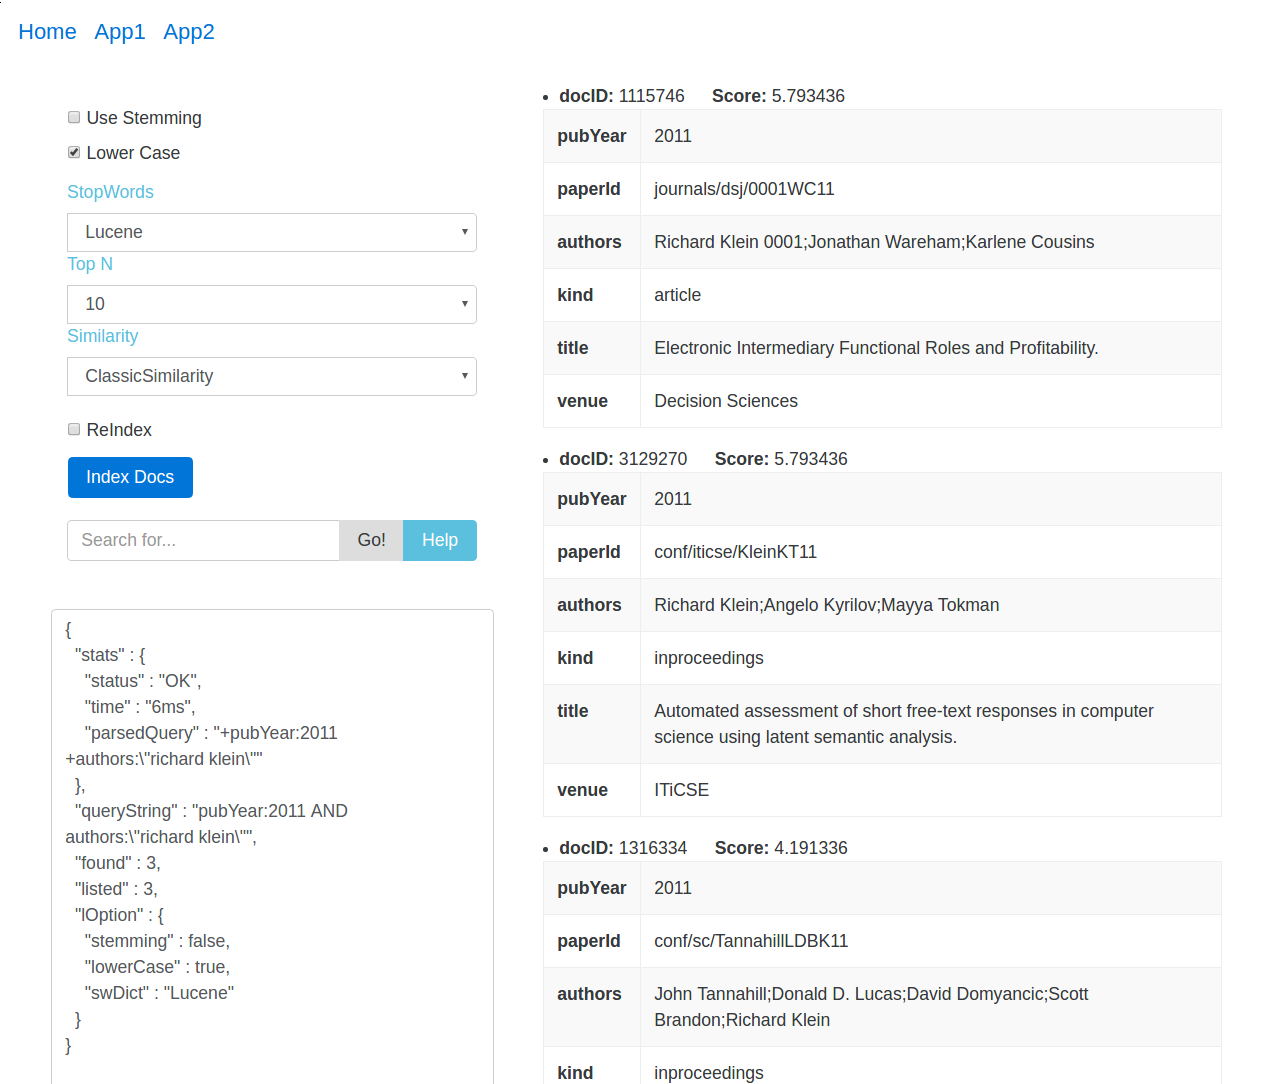
\includegraphics[width=\columnwidth]{ui.png}
  \cprotect\caption{LSearcher User Interface. This indicates a result for the query \verb|pubYear:2011 AND authors:"richard klein"|, the top-left is the control panel; bottom-left displays the action statistics; the right side displays the detailed results.}\label{fig:ui}
\end{figure}

The implementation consists of several parts.

\textbf{Data Extraction}. In order to extract the interesting data from DBLP database, we need to parse the XML and selectively generate publication records.

\textbf{Indexing}. Project 1 requires us to index each publication as a document; Application 2 in Project 2 requires an additional indexing on transactions or conference papers in a special year.

\textbf{Searching and Analyzing}. Project 1 and the two applications require to handle different kinds of queries, followed by analyses based on these results.

\textbf{Evaluation}. We need to conduct some experiments to evaluate the effectiveness and efficiency of the proposed tool.

Sections \ref{sec:extraction}$\sim$\ref{sec:proj2} will elaborate the approach as well as the core implementation with respect to these procedures.
